

\section{Weitere Datenstrukturen}


%------------------------------------------------------------------------------
\begin{frame}[fragile]{Graphenstruktur}
\metroset{block=fill}
  \begin{columns}[T,onlytextwidth]
    \column{0.37\textwidth}
    Anwendungen
      \begin{itemize}\footnotesize
          \item \textbf{Resource Description Framework (RDF):} 
          \begin{itemize}\footnotesize
              \item z.B. Blazegraph (Graph-DB)
              \item Abfrage: SPARQL
          \end{itemize}
          \item Labeled Property Graphs
          \begin{itemize}\footnotesize
              \item z.B. Neo4j (Graph-DB)
              \item Abfrage: Cypher
          \end{itemize}
      \end{itemize}
      
      \begin{block}{}
        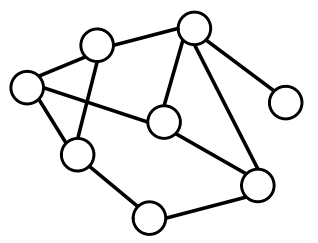
\includegraphics[width=0.97\textwidth]{img/graph.png}
      \end{block}


    \column{0.6\textwidth}
    RDF/Turtle-Notation (\texttt{.ttl})
\begin{turtlecode}
@prefix ex: <http://example.com/#> .

ex:Graz a ex:Ort;  
ex:name "Graz" ; 
ex:Einwohnerzahl 288806 ; 
ex:location [ ex:lat 47.4; ex:long 5.26 ] .

ex:Wien a ex:Ort;  
ex:name "Wien" ; 
ex:Einwohnerzahl 1897491 ; 
ex:location [ ex:lat 47.12; ex:long 16.22 ] .
\end{turtlecode}

SPARQL-Abfrage
\begin{sparqlcode}
@prefix ex: <http://example.com/#> .

SELECT ?name, ?einwohner
WHERE {
    ?ort ex:Einwohnerzahl ?einwohner .
}
\end{sparqlcode}

  \end{columns}
\end{frame}
%------------------------------------------------------------------------------


%------------------------------------------------------------------------------
\begin{frame}[fragile]{Baumstruktur: JSON}
%\metroset{block=fill}
    Anwendungen: \textbf{JavaScript Object Notation (JSON)}
          \begin{itemize}\footnotesize
              \item z.B. MongoDB
              \item keine standardisierte Abfragesprache, nur JavaScript 
          \end{itemize}

\begin{block}{}      
\begin{flushright}
        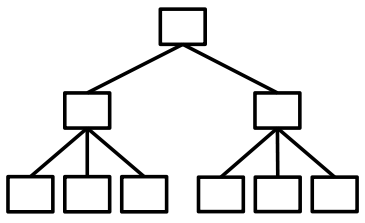
\includegraphics[width=0.25\textwidth]{img/baumstruktur.png}
\end{flushright}
\end{block}

JSON und JS (\href{https://www.w3schools.com/js/js_json_intro.asp}{w3s})
\begin{jscode}
'{"name": "John", "age": 30, "car": null, 
  "baum" : [
    "key": "value"
  ]
}'
const obj = JSON.parse('{"name":"John", "age":30, "city":"New York"}');
obj.age = obj.age.toString();
\end{jscode}

\end{frame}
%------------------------------------------------------------------------------


%------------------------------------------------------------------------------
\begin{frame}[fragile]{Baumstruktur: XML}
%\metroset{block=fill}
  \begin{columns}[T,onlytextwidth]
    \column{0.33\textwidth}
    Anwendungen: \textbf{eXtensible Markup Language (XML):}
          \begin{itemize}\footnotesize
              \item DBs: eXist, BaseX 
              \item Abfragesprachen: 
              XPath (\href{https://www.w3schools.com/xml/xpath_intro.asp}{w3s}) und XQuery (\href{https://www.w3schools.com/xml/xquery_example.asp}{w3s})
          \end{itemize}
          \bigskip

      \begin{block}{}
        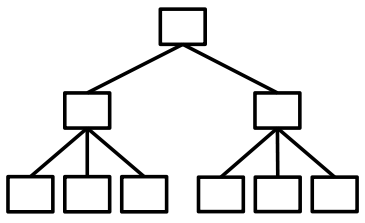
\includegraphics[width=0.95\textwidth]{img/baumstruktur.png}
      \end{block}

    \column{0.65\textwidth}
\begin{xmlcode}
<!-- books.xml -->
<?xml version="1.0" encoding="UTF-8"?>
<bookstore>
  <book>
    <title lang="en">Harry Potter</title>
    <author>J K. Rowling</author>
    <year>2005</year>
    <price>29.99</price>
  </book>
  <book>
    <title lang="en">Learning XML</title>
    <price>39.95</price>
  </book>
</bookstore>

<!-- XQuery -->
for $x in doc("books.xml")/bookstore/book
where $x/price>30
order by $x/title
return $x/title

<!-- XPath -->
//title[@lang='en']
/bookstore/book[price>35.00]
\end{xmlcode}

  \end{columns}
\end{frame}
%------------------------------------------------------------------------------

%------------------------------------------------------------------------------
\begin{frame}[fragile]{Webseiten}
%Datentypen, die man vielleicht kennen sollte
%\metroset{block=fill}
  \begin{columns}[T,onlytextwidth]
    \column{0.47\textwidth}
    HTML (\href{https://www.w3schools.com/html/default.asp}{w3s}) -- Struktur
\begin{htmlcode}
<!DOCTYPE html>
<html>
 <head>
   <title>Page Title</title>
 </head>
 <body>
  <h1>This is a Heading</h1>
  <p>This is a paragraph.</p>
 </body>
</html>
\end{htmlcode}

      
      \begin{block}{}
        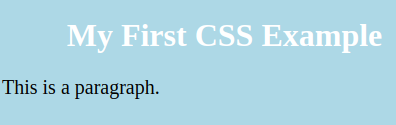
\includegraphics[width=0.97\textwidth]{img/css-example.png}
      \end{block}


    \column{0.47\textwidth}

CSS in HTML (\href{https://www.w3schools.com/css/default.asp}{w3s}) -- Darstellung
\begin{htmlcode}
<!DOCTYPE html>
<html>
  <head>
    <style>
body {
  background-color: lightblue;
}
h1 {
  color: white;
  text-align: center;
}
p {
  font-family: verdana;
  font-size: 20px;
}
    </style>
  </head>
  <body>
    <h1>My First CSS Example</h1>
    <p>This is a paragraph.</p>
  </body>
</html>
\end{htmlcode}

  \end{columns}
\end{frame}
%------------------------------------------------------------------------------


%------------------------------------------------------------------------------
\begin{frame}[fragile]{Tabellenstruktur: Relationale Datenbanken}
%\metroset{block=fill}
  \begin{columns}[T,onlytextwidth]
    \column{0.3\textwidth}
    Anwendungen
      \begin{itemize}\footnotesize
          \item z.B. SQLite, MySQL (Relationale Datenbanken) 
          \item Abfragesprache: SQL 
      \end{itemize}
      \bigskip 
      
      \begin{block}{}
        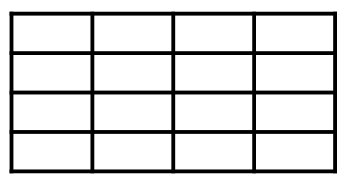
\includegraphics[width=0.97\textwidth]{img/tabelle.png}
      \end{block}


    \column{0.65\textwidth}
SQL-Abfrage
\begin{sqlcode}
CREATE TABLE "orte" (
 "name" TEXT,
 "einwohnerzahl" INTEGER,
 "breitengrad" REAL,
 "längengrad" REAL,
 PRIMARY KEY("name")
);

INSERT INTO orte 
VALUES 
('Graz', 288806, 47.066667, 15.433333), 
('Wien', 1897491, 48.208174, 16.373819);
\end{sqlcode}
\footnotesize
(name, einwohnerzahl, breitengrad, laengengrad) 

  \end{columns}
\end{frame}


%------------------------------------------------------------------------------
\begin{frame}[fragile]{3D-Datenformate Bsp \texttt{.ply}}

\begin{columns}
\footnotesize
  \column{0.35\textwidth}
  (\href{https://latex-ninja.com/2019/12/15/an-easy-intro-to-3d-models-from-structure-from-motion-sfm-photogrammetry/}{Blogpost zur Einführung in 3D/Structure from motion})

\begin{itemize}\scriptsize
    \item für 3D gibt es kein standardisiertes Datenformat
    \item \href{http://paulbourke.net/dataformats/ply/}{\texttt{.ply}} ist ein Beispiel der Umsetzung \\ `Polygon File Format' aka `Stanford Triangle Format'
    \item \href{http://paulbourke.net/dataformats/}{weitere Bsps siehe Link}
    \item 3D-Daten sind Koordinaten/Punkte im 3D-Raum (Meshes)
    \item mithilfe von Texturen kann man die Struktur bekommen
    \item nach Header und Metadaten folgt eine Tabelle mit 5 Spalten: \textbf{x, y, z, Farbe und Funktionswert}
\end{itemize}
  \column{0.62\textwidth}
  \tiny
  \metroset{block=fill}
  \begin{block}{}
  \begin{verbatim}ply
format ascii 1.0
comment author: Greg Turk
comment object: another cube
element vertex 8
property float x
property float y
property float z
property uchar red      { start of vertex color }
property uchar green
property uchar blue
element face 7
property list uchar int vertex_index { number of vertices per face }
element edge 5                       { five edges in object }
property int vertex1                 { index to first vertex of edge }
property int vertex2                 { index to second vertex }
property uchar red                   { start of edge color }
property uchar green
property uchar blue
end_header
0 0 0 255 0 0           { start of vertex list }
0 0 1 255 0 0
0 1 1 255 0 0
0 1 0 255 0 0
1 0 0 0 0 255
1 0 1 0 0 255
1 1 1 0 0 255
1 1 0 0 0 255
3 0 1 2                 { start of face list, begin w/ triangle }
3 0 2 3                 { another triangle }
4 7 6 5 4               { now some quadrilaterals }
\end{verbatim}
  \end{block}
\end{columns}

\end{frame}
%------------------------------------------------------------------------------


%------------------------------------------------------------------------------
\begin{frame}[fragile]{3D-Datenformate Bsp \texttt{.ply} (Fortsetzung)}

\begin{columns}
\footnotesize
  \column{0.35\textwidth}
  (\href{https://latex-ninja.com/2019/12/15/an-easy-intro-to-3d-models-from-structure-from-motion-sfm-photogrammetry/}{Blogpost zur Einführung in 3D/Structure from motion})

\begin{itemize}\footnotesize
    \item nach Header und Metadaten folgt eine Tabelle mit 5 Spalten: \textbf{x, y, z, Farbe und Funktionswert}
    \item der Funktionswert = Ergebnis einer Funktion, z.B. Farbgradient, wird immer überschrieben
    \item Öffnen z.B. in Blender, AutoCAD, Meshlab
\end{itemize}
  \column{0.6\textwidth}
  \tiny
  \metroset{block=fill}
  \begin{block}{}
  \lbrack{}continued\rbrack{}
  \begin{verbatim}
4 7 6 5 4       { now some quadrilaterals }
4 0 4 5 1
4 1 5 6 2
4 2 6 7 3
4 3 7 4 0
0 1 255 255 255 { start of edge list, begin with white edge }
1 2 255 255 255
2 3 255 255 255
3 0 255 255 255
2 0 0 0 0       { end with a single black line }
\end{verbatim}
  \end{block}
\end{columns}

\end{frame}
%------------------------------------------------------------------------------


%------------------------------------------------------------------------------

